\documentclass[11pt,a4paper]{article}

\usepackage{fullpage}
\usepackage{hyperref}
\usepackage{graphicx}

\usepackage{caption}
\usepackage{subcaption}
\usepackage{spverbatim}

\usepackage{float}

\usepackage{fancyhdr}
\pagestyle{fancy}
\fancyhf{}
\usepackage{todonotes}                %% notes from the authors

\renewcommand{\headrulewidth}{0pt}
\renewcommand{\footrulewidth}{0pt}

\fancypagestyle{firstpagefooter} {
	\lfoot{\tiny{Version: 25.09.2018}}
	\cfoot{}
	\rfoot{\thepage}
	
}

\lfoot{Name: David Yenicelik Legi: 15-944-366}
\rfoot{\thepage}

\begin{document}

\title{Advanced Systems Lab Report\\ \normalsize{Autumn Semester 2018}}
\author{Name: David Yenicelik \\Legi: 15-944-366}
\date{
	\vspace{4cm}
	\textbf{Grading} \\
	\vspace{0.5cm}
	\begin{tabular}{|c|c|}
		\hline  \textbf{Section} & \textbf{Points} \\
		\hline  1                &                 \\ 
		\hline  2                &                 \\ 
		\hline  3                &                 \\ 
		\hline  4                &                 \\ 
		\hline  5                &                 \\ 
		\hline  6                &                 \\ 
		\hline  7                &                 \\ 
		\hline \hline Total      &                 \\
		\hline 
	\end{tabular} 
}
\maketitle
\thispagestyle{firstpagefooter}

\newpage

\section*{Notes on writing the report \small{(remove this page for submission)}}

Furthermore, it is expected that the interactive law holds for all experiments. In case throughput and response time do not match, it is imperative that you explain why, otherwise you risk losing most of the points for the experiment in question.

In each section you can find a table summarizing the system configuration that should to be used for that particular section. These configurations should be considered as a guideline to help you find interesting configurations where we expect your system to change its behaviour (e.g., going from an under-saturated to a saturated system). If you do not observe such a change inside that range of parameters, you should expand the range and run additional experiments outside the given range. In that case, ask your assistant for advise.

This document provides you with the end-results that have to be included in the report. Please keep in mind that you are encouraged to provide additional graphs and experiments that help you in understanding your system. These additional experiments should be chosen such that they support the claims you make in your explanations and help you illustrate your point.


\subsection*{How to Generate Load and Populate the Data}

To generate load on the system, you will use memtier. When using memtier, you can specify two parameters: the number of threads (CT) and the number of virtual clients per thread (VC). The total number of virtual clients per memtier is CPM=CT*VC. When referring to ``number of clients'' in the system, it is the number of memtier instances times the number of virtual clients per instance, i.e., NumClients=NumMemtier*CPM.

Increasing NumClients for experiments is always done by first fixing the number of virtual machines (VMs) and memtier instances and then changing the VC setting for all memtiers. In most cases it is enough to increase VC in large increments, unless you want to explore the behavior of your system around the inflexion point or other points which are of interest. In this case, you can use more fine-grained steps.

For all experiments, use 2 CT per VM and between 1 and 32 VC per thread. We recommend to choose at least 6 points in this range. You will have to use up to 3 VMs for clients. In case you use a single middleware, set up each memtier instance with 2 CTs. If you use two middlewares, start two memtier instances per VM (each connected to one middleware) with 1 CT each.

For all experiments conducted in this report, the value size has to be 4096\,Bs, and the number of keys 10000 (\texttt{--key-maximum=10000}). Before running experiments, populate the key-value store using a write-only workload long enough to write all keys at least once. All sets should have a long expiry time, to ensure that keys are not evicted during the experiments (e.g., \texttt{--expiry-range=9999-10000}). The loading of the memcached servers is not part of the measured performance, and the middleware has to be restarted after the initial population, before running experiments. 

\subsection*{Plotting Data}
The readability of your grades will be part of the grade. For all graphs the y-axis should start at 0, always use appropriate error metrics/bars, label both axis with units. For graphs that are related try to keep the same range on the x- and y-axis. Be careful when using log-scale on any of the axis. 
\newpage

\section{System Overview (75 pts)}

I structure my project (code only) into the following folders.
I give a short explanation for each item on how it is used.

I will start out with a diagram that explains the overall structure and refers to each .java file.
I will then be more detailed with my project-code structure.

\begin{figure}[H]
\centering
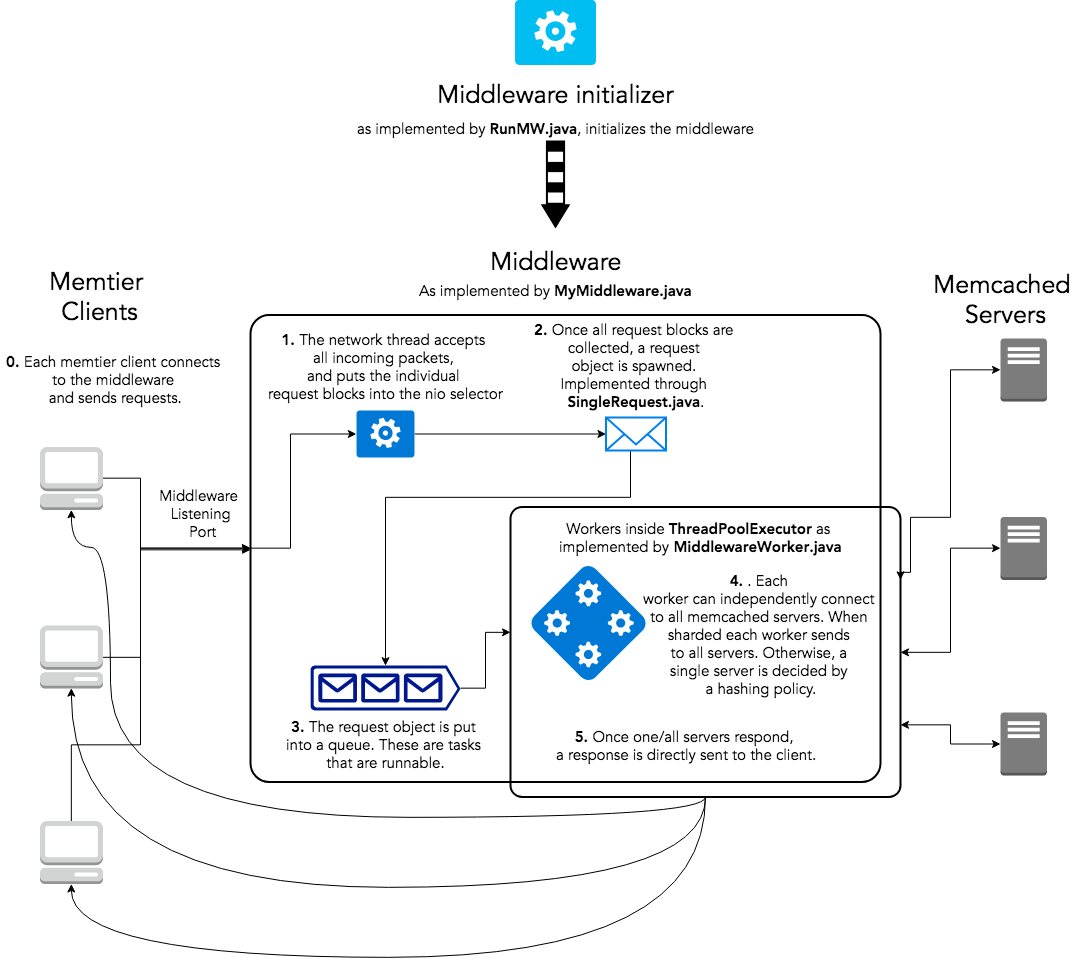
\includegraphics[width=\textwidth]{img/middleware_diagram.png}
\caption{Exp.2.1: A figure with two subfigures}
\label{fig:test}
\end{figure}


\begin{enumerate}
\item \textbf{scripts} \\
This folder includes all the logic to automatically compile the code, deploy the code, run the experiments (each individual one), and automatically download the logs.
This is true both for a local development environment (using docker VM's), and the external "production" environment (using Azure VM's). 
The local docker and external Azure systems are interchangable with a small change in command.

\item \textbf{data} \\
This folder includes all the raw data that is pulled from the experiment, all the python files which process upon this data, and all the processed data.

\item \textbf{figs} \\
This folder includes all the figures that are create using the processed data from point 2.
I use python to create figures from individual graphs

\item \textbf{src} \\
I will talk about the code structure of the src directory with more detail in this next section.
I take a top-down approach while explaining (i.e. starting with where requests originate, and where they go from there).
I will keep this consice, as the \textit{lifetime of a request} section covers some information on what happens in which file.

\begin{enumerate}
\item \textbf{RunMW.java} \\
This is the entry point / main class of the program.
This is the default implementation by the TA's.


\item \textbf{SingleRequest.java} \\
Is the class which encodes a single request from one of the clients.
This can include the SET or GET operation.
For logging purposes, this class also includes all possible times which may be of use to calculate the queueing theory (and latency and throughput) later on.

The request type is parsed by checking the very first character of the request string.
If the string starts with a "g", the request type is a GET (later on, it is decided on the fly if it is a MULTIGET by checking if the number of keys is greater than 1).
If the string starts with a "s", the request type is a SET.
If none of the above cases hold, an error happened (we exit gracefully, as this is unintended behavior).

\item \textbf{MyMiddleware.java} \\
This is the entrypoint of how the Middleware is called.
The datastructure we use to connect to the individual clients is the \textbf{nio.Selector}. 
The \textbf{nio.Selector} can hold multiple connections from different clients conneting. 
Furthermore, it can parse packages that don't immediately fit into the bytebuffer 

This class is responsible for fetching the individual requests (spawned as a \textit{SingleRequest} object)using non-blocking IO, putting it to a queue, and spawning \textit{MiddlewareWorker}'s within a \textit{ThreadPool} to act upon these requests.
We use the NIO selector to handle all connections.
The entire logic of this .java class runs in on the main thread of the class, which I may refer to as "Network Thread".
This allows for multiple clients to connect to the server in a non-blocking fashion.
Whenever a connection is compelte (i.e. the request is complete), this selector spawns a \textit{MiddlewareWorker} and a \textit{SingleRequest}.

The following diagram symbolizes how this works.

\item \textbf{MiddlewareWorker.java} \\
The \textit{MiddlewareWorker} takes a \textit{SingleRequest} and passes it to the server(s). 
The \textbf{MiddlewareWorker} implements \textbf{Runnable}, and is executed by the \textbf{ThreadPoolExecutor} by calling \textbf{submit}.
Depending on whether the request type is a SET or GET, we have different behavior:

\begin{itemize}
\item case SET: 
The \textit{SingleRequest} is sent to each individual server in a sequential manner.
After the sending to the server is done for all servers, it listens to the response of each individual server.
It listens until all servers have responded.
If any single item has responded with an error, this SET operation responds with the first error encountered to the client.
Otherwise it returns a \textbf{STORED} message. 

\item case GET: 
The string of the \textit{SingleRequest} is used to calculate a hash for the individual request.
This hash is then modulo-ed with the number of server that we can send the request to.
The modulo operation decides which server to send it to.
This has \textbf{provenly uniformly at random distribution}  behavior (proof at: \href{https://eprint.iacr.org/2016/985.pdf, https://en.wikipedia.org/wiki/K-independent_hashing, https://www.akamai.com/es/es/multimedia/documents/technical-publication/consistent-hashing-and-random-trees-distributed-caching-protocols-for-relieving-hot-spots-on-the-world-wide-web-technical-publication.pdf}).
In short, this proof relies on the fact that hashing is pseudorandom, and that pseudorandomity is means that for any input, all output values are uniformly at random distributed.

\item case MULTIGET (nonsharded):
The nonsharded multiget acts exactly like the GET case.
Again, the uniformly at random assumption is guaranteed because the hashing algorithm is pseudorandom (and as such provides keys uniformly at random).

\item case MULTIGET (sharded):
The sharded MULTIGET case acts as follows. The MULTIGET request is first split up into $n = max(keys, buckets)$ where $buckets$ is the number of servers in total, and $keys$ is the number of keys in total.
Each individual split up request is then treated as an individual GET request.
When the memcached server responds, all the answers are concatenated in a sequential fashion and sent back to the client.
\end{itemize}


\item \textbf{LoggerUtils.java} \\
A helper class.
Includes all the logic that is needed to log the requests to hard disk.
All the request logic is accumulated to a list, and at the very end, flushed to disk (using this logger class and some logic from the middleware worker).
The logging happens in such a way that each individual \textit{MiddlewareWorker} has it's list of requests to be logged at.
Once no more incoming requests get in for more than a few seconds (as decided by the \textit{MyMiddleware}), all the logs are flushed to disk (and then downloaded to local for further processing).
This way, there are no issues with multithreading as there is no concurrent data access. \\

Every single request keeps track of the following values, 
which is then flushed to the LoggerUtils.java (and thus to the file)
object when the request has been successfully.

\begin{enumerate}
\item timeRealOffset
\item differenceTimeCreatedAndEnqueued
\item differenceTimeEnqueuedAndDequeued
\item differenceTimeDequeuedAndSentToServer
\item differenceTimeSentToServerAndReceivedResponseFromServer
\item differenceTimeReceivedResponseFromServerAndSentToClient
\item timeRealDoneOffset
\end{enumerate}

\item \textbf{RequestType.java} \\
A helper struct definition, which defines the two possible input types (Multi-gets are decided on the fly at a different point)

\end{enumerate}

\end{enumerate}

\subsection{Lifetime of a request}
In the following I will talk about how requests enter the middleware, how they are parsed, how they get distributed to servers, and how the middleware communicates these values back to the clients. \\

\begin{enumerate}
\item \textbf{Request coming from client to middleware:}\\
When a request comes from a client to the middleware, I use an \textbf{nio.channels.Selector} to accept the request.
This datastructure has the following benefits.
First, it can distinguish between multiple clients.
Second, it can process these individual requests simultaneously in an asynchronous (non-blocking) manner.
Third, it fills up multiple channels (one for each connection, and thus, one for each client), which means that if the request does not fit into one network packet, it will just listen for the rest of the packet.
I detect if a single request fills up by filling a java \textbf{ByteBuffer} until it the request has come to an end (which we can recnognize by waiting for the \textbf{END} keyword.
We parse the type of request by looking at the very first character (interpreting the bytes) and cross-comparing if this is a \textit{set} or \textit{get}. 
To distinguish between \textit{multi-get} and \textit{gets}, we later on split the string resulting from parsing the bytebuffer by spaces.
If the number of elements after splitting is bigger than 2 (the "get" keyword, and the key), then I parse a multi-get.
Else, I parse a get.
\item \textbf{The incoming request spawns a SingleRequest object:}\\
The SingleRequest object is specified in the \textbf{SingleRequest.java} java file and implements a java \textbf{Runnable} on which I later on call \textbf{submit} using a \textbf{ThreadPoolExecutor}. 
This file keeps track of the statistics described in the LoggerUtils.java class for logging.
The SingleRequest takes over the \textbf{ByteBuffer} which was created while \textbf{nio.channels.Selector} was listening for a complete network packet.
This ByteBuffer will later on be passed to the individual server(s) (after some processing).
\item \textbf{Submitting a SingleRequest to a MiddlewareWorker using the java ThreadPoolExecutor}:\\
I use the SingleRequest that was generate before, and spawn a new MiddlewareWorker.
This MiddlewareWorker can then be submitted to the java \textbf{ThreadPoolExecutor} which contains the number of middleware-threads (as specified per experiment).
Each individual middlewareworker contains one instantiated \textbf{LoggerUtils} class per thread and thus is threadsafe.
\item \textbf{Sending the server response back to the client}: \\
The response is sent back to the client using the description in the previous sub-section.
In any case, this goes through the individual middleware-worker thread, and does \textbf{not} go through the initial nio.channel.Selector again.
\end{enumerate}

\subsection{General numbers observed w.r.t. clients, middlewares and server}
Some general observations include the following approximate maximum throughput. 
I did not include graphs to this, as all these experiments just involve scalars. \\

Each VM in the azure network has a maximum throughput of approximately 200Mbit/s (between 215 and 192Mbit/s) as determined by the program \textbf{iperf}.
Because we are dealing with packages of size 4096 bytes (i.e. 4kbytes or 32 Kbits), this means that there the maximum upload capacity of a single virtual machine is approximately $$ \frac{200Mbit/s}{32Kbit} \approx 6'250 ops/s$$.\\

Intuitively, this means that if we have 3 clients and one server, the server must be a bottleneck, and that the clients share the $6'250 ops/s$ (approximately $2'000ops/s$ per client).
I will use these numbers to derive some explanations later on.\\

For all experiments, I will take the mean and standard deviation amongst three individual trials / repetitions.
The mean $\mu$ and standard deviation ($\sigma$) are calculated as follows:

\begin{equation}
\mu = \frac{\sum_i^n x_i} {n}
\end{equation}

\begin{equation}
\sigma = \sqrt{ \frac{\displaystyle\sum_{i=1}^{n}(x_i - \mu)^2} {n} }
\end{equation}



%TODO 
\textbf{??????}
Include illustrations that show how requests of different types are handled (e.g., components involved in processing the request and method calls). 

\section{Baseline without Middleware (75 pts)}
These experiments don't use the middleware, and only consist of memtier client instances, and memcached server instances.

\subsection{One Server}

\begin{center}
	\scriptsize{
		\begin{tabular}{|l|c|}
			\hline Number of servers                & 1                        \\ 
			\hline Number of client machines        & 3                        \\ 
			\hline Instances of memtier per machine & 1                        \\ 
			\hline Threads per memtier instance     & 2                        \\
			\hline Virtual clients per thread       & [1..32]                  \\ 
			\hline Workload                         & Write-only and Read-only \\
			\hline Repetitions                      & 3 or more                \\ 
			\hline 
		\end{tabular}
	} 
\end{center}

I will test out the response time and latency for a different number of virtual clients per thread on the client-side (per memtier instance), namely [1, 2, 4, 8, 16, 32].
I will have two different subsections for read-only operations, and write-only operations.
As there is no difference in pre-populating the servers in the case of writes, for both experiments I pre-populate the server the same way as in experiment 2.1 (Baseline without middleware and 3 clients).
The clients and servers don't use multi-gets, and there is no middleware involved.
I run 3 repetitions of each configuration, each having a length of 90 seconds (such that the warm-up and cool-down times even out).

For read-only workloads, I pre-populate the server using the following memtier command. 
In future, if I ever refer to populating the server(s), I use this same command:
\begin{spverbatim}
      memtier_benchmark -s {SERVER_IP} -p {PORT}
      --protocol=memcache_text --clients={VIRTUAL_CLIENTS_PER_THREAD} --threads={THREADS}
      --requests=15000 --ratio=1:0 --data-size=4096
     --expiry-range=9999-10000 --key-maximum=10000 --key-pattern=S:S
\end{spverbatim}

I run 3 repetitions of each configuration, each having a length of 90 seconds (such that the warm-up and cool-down times even out).

\subsubsection{Read-only}

I first present the graph. 
The throughput reached approximately almost $3000ops/s$, which conforms to the observation of the maximum throughput per server in section 1. 

\begin{figure}[H]
\centering
\begin{subfigure}{.5\textwidth}
    \centering
    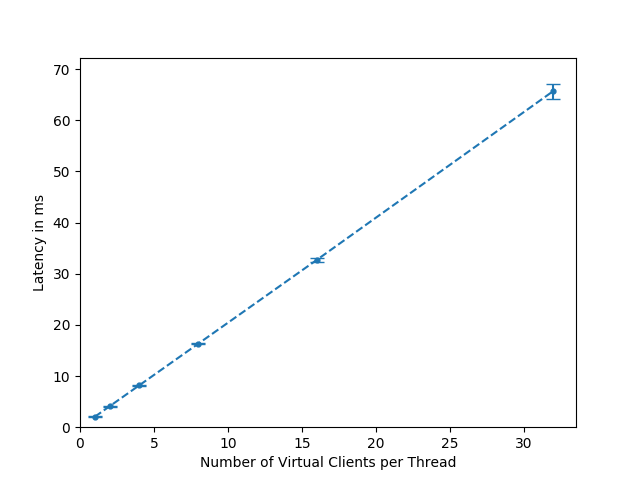
\includegraphics[width=\textwidth]{img/exp2_1/exp2_1_latency_write_0.png}
    \caption{Response time / Latency in ms per single request}
    \label{fig:mesh1}
\end{subfigure}%
\begin{subfigure}{.5\textwidth}
      \centering
    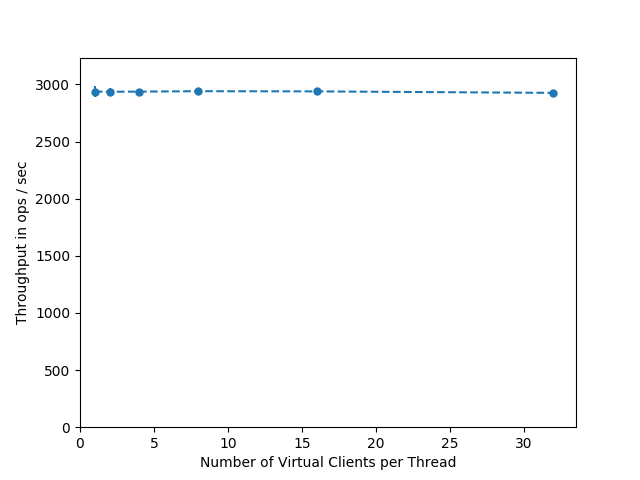
\includegraphics[width=\textwidth]{img/exp2_1/exp2_1_throughput_write_0.png}
    \caption{Total throughput pre}
    \label{fig:mesh1}
\end{subfigure}
\caption{Experiment 2.1, Baseline without middleware and one server. Read-only latency and throughput per individual client (mean $+/-$ standard deviation)}
\label{fig:test}
\end{figure}

For read-only operations, the bottleneck is the upload bandwidth of the server,
as 3 clients are trying to download a load of 200Mbit/s, and thus must each share appr. 66Mbit/s.
The total upload bandwidth of 6000ops/sec (which was empirically proven in section 1 through an additional experiment), is thus divided amongst  three servers.
The clients are able to generate enough load with even 1 virtual thread, such that with 1 virtual thread the network bandwidth is saturated.
As the number of threads increases, more requests are able to be generated.
Because the network bandwidth stays constant, the round-trip time of individual requests increases.
This implies an increase in latency, as can be seen from the graph.


The latency increases linearly.

\subsubsection{Write-only}
Again, I first present the graph.
The throughput reached approximately almost $18000ops/s$, which is conforms to the observation of the maximum throughput per server in section 1.

\begin{figure}[H]
\centering
\begin{subfigure}{.5\textwidth}
    \centering
    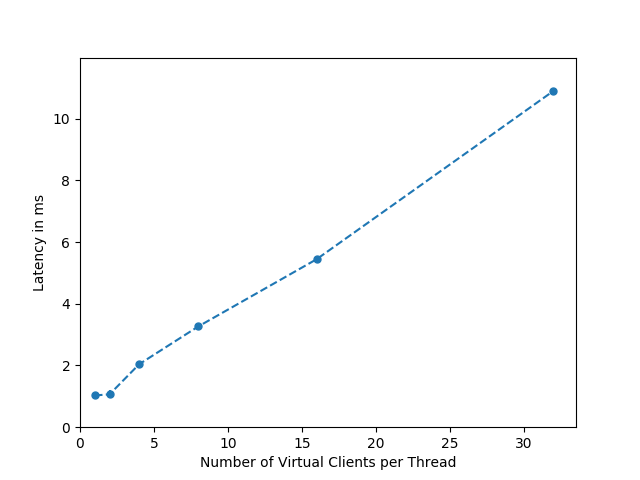
\includegraphics[width=\textwidth]{img/exp2_1/exp2_1_latency_write_1.png}
    \caption{Latency write only}
    \label{fig:mesh1}
\end{subfigure}%
\begin{subfigure}{.5\textwidth}
      \centering
    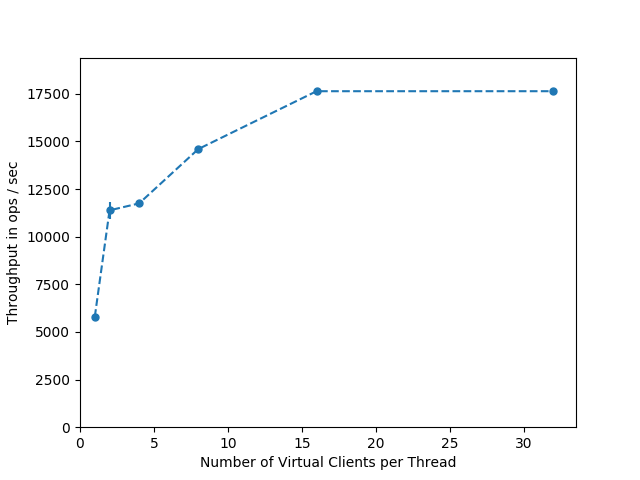
\includegraphics[width=\textwidth]{img/exp2_1/exp2_1_throughput_write_1.png}
    \caption{Throughput write only}
    \label{fig:mesh1}
\end{subfigure}
\caption{Exp.2.1: A figure with two subfigures}
\label{fig:test}
\end{figure}

The single server is fast enough to respond to all individual client requests, as the server is only responding with the message "STORED" each time.
However, at some point, the number of requests is so high, that either the individual client output bandwidth, or storing the actual requests on the hard-ware side becomes the bottleneck.
This can be seen as the throughput grows square-root like, and then saturates.
The throughput graph, which means out with 16 virtual clients per thread, proves this point.
To decide whether the network is the bandwidth is the bottleneck, I repeat this experiment locally with virtual docker containers.
These plateau at a later stage, which proves that the maximum network bandwidth is reached with 16 virtual clients per thread.

%TODO :
Latency and throughput correlate in the following way: \textbf{???}

\subsection{Two Servers}

For the following experiment, I use the following setup:

\begin{center}
	\scriptsize{
		\begin{tabular}{|l|c|}
			\hline Number of servers                & 2                        \\ 
			\hline Number of client machines        & 1                        \\ 
			\hline Instances of memtier per machine & 2                        \\ 
			\hline Threads per memtier instance     & 1                        \\
			\hline Virtual clients per thread       & [1..32]                  \\ 
			\hline Workload                         & Write-only and Read-only \\
			\hline Repetitions                      & 3 or more (at least 1 minute each)                \\ 
			\hline 
		\end{tabular}
	} 
\end{center}

I will test out the response time and latency for a different number of virtual clients per thread on the client-side (per memtier instance), namely [1, 2, 4, 8, 16, 32].
I will have two different subsections for read-only operations, and write-only operations.
As there is no difference in pre-populating the servers in the case of writes, for both experiments I pre-populate the server the same way as in experiment 2.1 (Baseline without middleware and 3 clients).
The clients and servers don't use multi-gets, and there is no middleware involved.
I run 3 repetitions of each configuration, each having a length of 90 seconds (such that the warm-up and cool-down times even out).

\subsubsection{Read-only}

I first present the graph. 
The throughput reached approximately almost $6000ops/s$, which conforms to the observation of the maximum throughput per virtual machine in section 1.
This means that the client virtual machine is using its maximum capacity to download all the values that are uploaded by the server virtual machines.


\begin{figure}[H]
\centering
\begin{subfigure}{.5\textwidth}
    \centering
    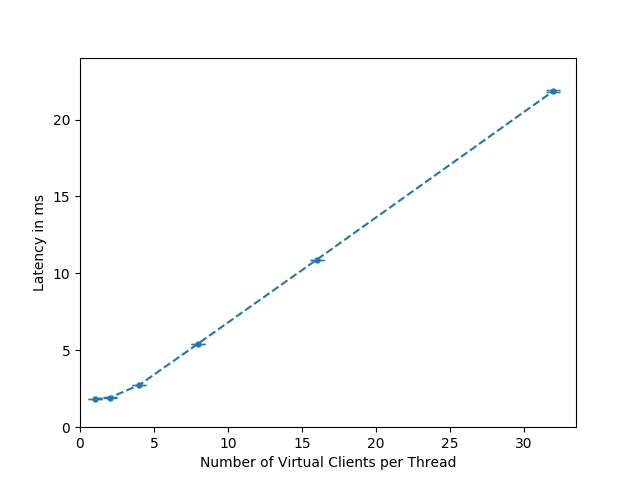
\includegraphics[width=\textwidth]{img/exp2_2/exp2_2__latency_write_0.png}
    \caption{Exp2.2: Latency read only}
    \label{fig:mesh1}
\end{subfigure}%
\begin{subfigure}{.5\textwidth}
      \centering
    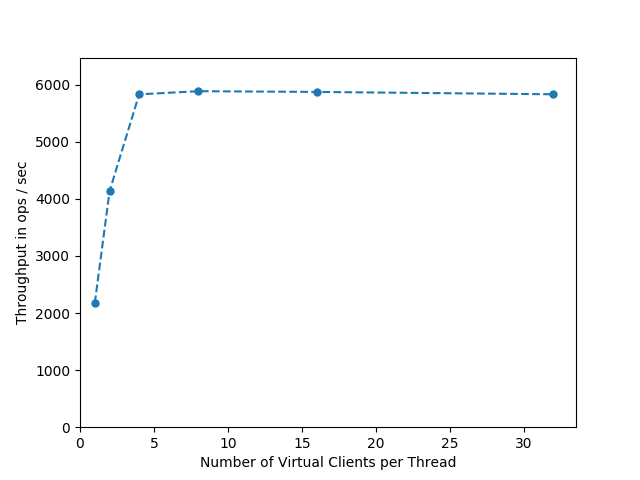
\includegraphics[width=\textwidth]{img/exp2_2/exp2_2__throughput_write_0.png}
    \caption{Throughput read only}
    \label{fig:mesh1}
\end{subfigure}
\caption{Exp2.2: A figure with two subfigures}
\label{fig:test}
\end{figure}

For read-only operations, the bottleneck is the download bandwidth of the client virtual machine,
as 1 client is trying to download 200Mbit/s.
The total upload bandwidth of 6000ops/sec (which was empirically proven in section 1 through an additional experiment), is thus divided amongst amongst two memtier servers.
The clients are able to generate enough load with even 1 virtual thread, such that with 1 virtual thread the network bandwidth is saturated.
The system does not become instable after an increase of virtual client threads, as can be seen from the plot which indicates that there is no oversaturation (there is a saturation phase instead).
As the number of threads increases, more requests are able to be generated.
Because the network bandwidth stays constant, the round-trip time of individual requests increases.
This implies an increase in latency, as can be seen from the graph.
The latency and throughput graphs show a correct, inverse correlation.

\subsubsection{Write-only}

Again, I first present the graph.
The throughput reached approximately almost $12000ops/s$, which conforms to the observation of the maximum throughput per virtual machine (in this case the server) in section 1.

\begin{figure}[H]
\centering
\begin{subfigure}{.5\textwidth}
    \centering
    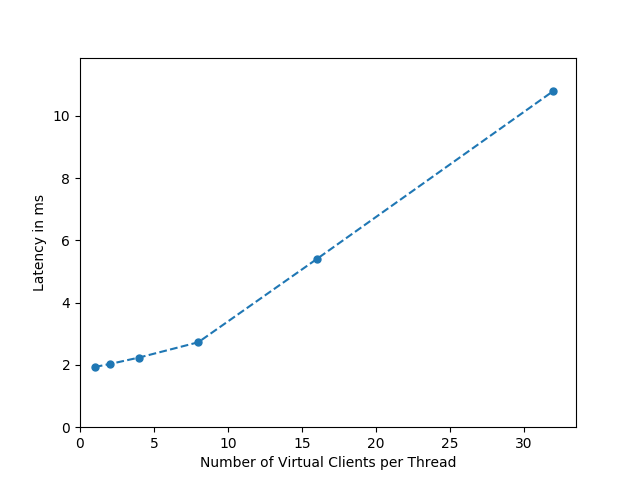
\includegraphics[width=\textwidth]{img/exp2_2/exp2_2__latency_write_1.png}
    \caption{Latency write only}
    \label{fig:mesh1}
\end{subfigure}%
\begin{subfigure}{.5\textwidth}
      \centering
    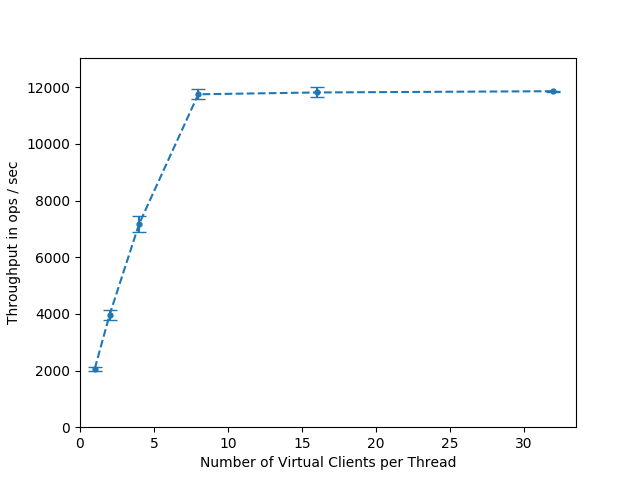
\includegraphics[width=\textwidth]{img/exp2_2/exp2_2__throughput_write_1.png}
    \caption{Throughput write only}
    \label{fig:mesh1}
\end{subfigure}
\caption{A figure with two subfigures}
\label{fig:test}
\end{figure}

The two servers are fast enough to save all the set requests.
The download speed of the individual servers virtual machines can handle enough requests until 8 virtual client threads.
One can see this for that the graph shows a plateau, which indicates a saturation phase at 8 virtual client threads.
The upload bandwidth of the client is also sufficient to populate the individual servers, until the two servers cannot respond to the individual requests any faster.
The single server is fast enough to respond to all individual client requests, as the server is only responding with the message "STORED" each time.
However, at some point, the number of requests is so high, that either the individual client output bandwidth, or storing the actual requests on the hard-ware side becomes the bottleneck.
This can be seen as the throughput grows square-root like, and then saturates.
The throughput graph, which means out with 8 virtual clients per thread, proves this point.
To decide whether the network is the bandwidth is the bottleneck, I repeat this experiment locally with virtual docker containers.
These plateau at a later stage, which proves that the maximum network bandwidth is reached with 16 virtual clients per thread. \\

Latency and throughput correlate in the following way. 
The latency is inversely proportional to the throughput.
One can see clearly that this explanation is supported by the two graphs, which show that overall trend of the latency is exponential, while the overall trend of the throughput is logarithmic.
These are inverse functions of each other.

\subsubsection{Explanation}

TODO: compare two-servers and one-server approaches.

Describe how this experiment compares to the previous section. Which results are the same and which ones differ? Explain what further conclusions can be drawn from the experiment.


\subsection{Summary}

Based on the experiments above, fill out the following table:

%TODO : Get exact values from the experiments

\begin{center}
	{Maximum throughput of different VMs.}
	\begin{tabular}{|l|p{2cm}|p{2cm}|p{4cm}|}
		\hline                        & Read-only workload & Write-only workload & Configuration gives max. throughput \\ 
		\hline One memcached server   & 1  / 2938 & 16 / 14595 & VC=16  \\ 
		\hline One load generating VM & 4  / 5872 & 8 / 11859 & VC=8 \\ 
		\hline 
	\end{tabular}
\end{center}

We can compare the read-only and write-only workloads.
The write-only workloads have higher throughputs compared to the read-only workloads.
Also, the configuration with only a single memcached server has higher spread, which means that $17500 - 2900 = 14600$ is higher than $12000 - 5800 = 6200$. 
This is because we change it from one server to two servers, whereas we reduce the number of clients from 3 to 1.
The change of number of clients has higher effect.
In addition to that, saturation is reached much faster with only a single load-generating client, as all get and set request bodies (i.e. the data) has to enter and leave this VM.
This means that in the load-generating VM, the single memtier client is the bottleneck.
In the case of one memcached server, the bottleneck is the server (read only case), which has to respond with the response bodies and thus the maximum upload bandwith (bottleneck) is reached.
In the case of one memcached server write-only case, the bottleneck is the clients which have to send the request bodies.
Each client has a maximum bandwidth of 6000 ops/sec.

\section{Baseline with Middleware (90 pts)}

In this set of experiments, I use three client memtier virtual machines, and 1 memcached server.
These virtual machine instances are connected with exactly one middleware virtual machine in the middle.
The three clients connect to the middleware. 
The middleware connects to the server.

The general tendency is that read-only requests are just as fast,
while write-only requests are a bit slower and occur over-saturation in the middleware (probably due to the buffer sizes).

\subsection{One Middleware}

\begin{center}
	\scriptsize{
		\begin{tabular}{|l|c|}
			\hline Number of servers                & 1                        \\ 
			\hline Number of client machines        & 3                        \\ 
			\hline Instances of memtier per machine & 1                        \\ 
			\hline Threads per memtier instance     & 2                        \\
			\hline Virtual clients per thread       & [1..32]                  \\ 
			\hline Workload                         & Write-only and Read-only \\
			\hline Number of middlewares            & 1                        \\
			\hline Worker threads per middleware    & [8..64]                  \\
			\hline Repetitions                      & 3 or more (at least 1 minute each)                \\ 
			\hline 
		\end{tabular}
	} 
\end{center}

The setup is exactly the same as in experiment "Baseline without Middleware and 1 server", with the difference that we inject one middleware between the 
clients, and the server.

In addition the measuring the throughput and response time for different values of number of virtual clients, we also allow to modify the number of middleware threads as another measureable variable.
This means that I test out the throughput and latency for any permutation of
virtualthreads=[1, 2, 4, 8, 16, 32] and threads in the middleware=[8, 16, 32, 64].
I repeat each experiment for 3 times and plot the standard deviation amongst those trials.
I also allow for a 15 second warm-up and 15 second cool-down time, and disregard these measurements when retrieving the logs about the request times from the middleware.\\

The throughput reached approximately almost $3000ops/s$, which conforms to the observation of the maximum throughput per server in section "Baseline without Middleware and 1 server". \\

\subsubsection{Read-only and Explanation}
I will first plot the latency (response time) and the throughput as measured on the middleware.
I will the show some plots generated by the logs of the client-machine which underline a correct measurement.

\begin{figure}[H]
\centering
\begin{subfigure}{.5\textwidth}
    \centering
    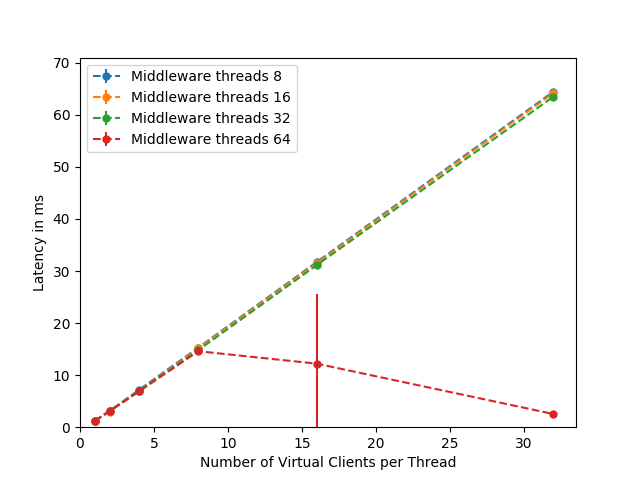
\includegraphics[width=\textwidth]{img/exp3_1/exp3_1__latency_middleware_write_0.png}
    \caption{Exp2.2: Latency read only}
    \label{fig:mesh1}
\end{subfigure}%
\begin{subfigure}{.5\textwidth}
      \centering
    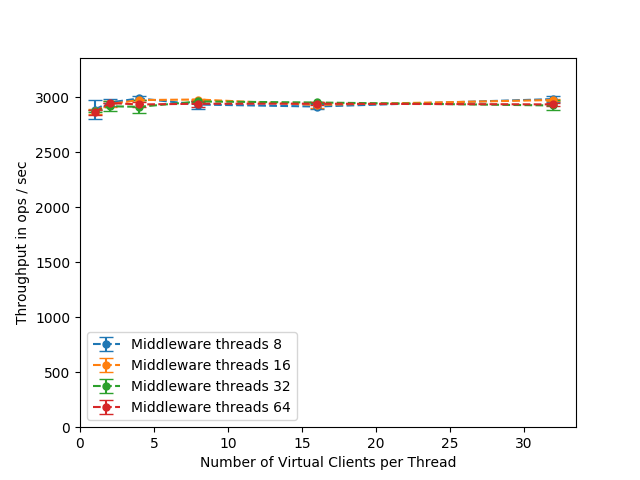
\includegraphics[width=\textwidth]{img/exp3_1/exp3_1__throughput_middleware_write_0.png}
    \caption{Throughput read only}
    \label{fig:mesh1}
\end{subfigure}
\caption{Exp3.1: Latency and throughputs as measures by the \textbf{middlewares}}
\label{fig:test}
\end{figure}

For read-only operations, the bottleneck is the upload bandwidth of the server,
as 3 clients are trying to download a load of 200Mbit/s, and thus must each share appr. 66Mbit/s.
The middleware virtual machine does not slow this down, as all GET requests are very short simple requests that all fit into the buffer.
The total upload bandwidth of 6000ops/sec (which was empirically proven in section 1 through an additional experiment), is thus divided amongst  three servers.
The clients are able to generate enough load with even 1 virtual thread, such that with 1 virtual thread the network bandwidth is saturated.
As the number of threads increases, more requests are able to be generated.
Because the network bandwidth stays constant, the round-trip time of individual requests increases.
This implies an increase in latency.
The linear increase in the latency graph supports this. \\

As a sanity check, I present the throughput and latency plots from the client machines, which all conform to the throughputs and latencies as caluclated in the middleware.
Another sanity check is that the interactive law holds, which states that the response-time \textbf{per request}  is related inversely-linearly proportional to the throughput.

\begin{figure}[H]
\centering
\begin{subfigure}{.5\textwidth}
    \centering
    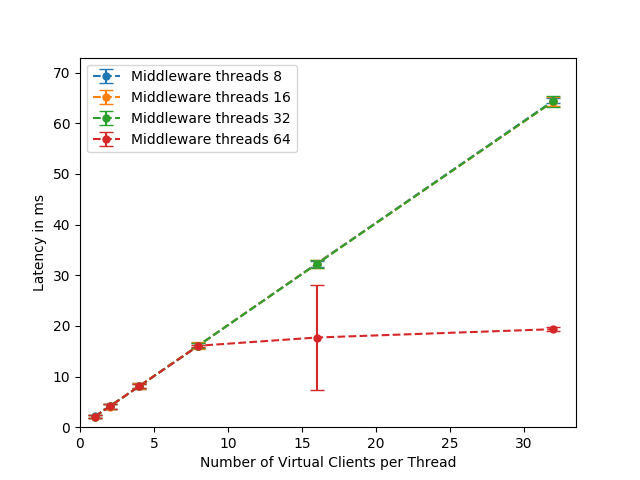
\includegraphics[width=\textwidth]{img/exp3_1/exp3_1__latency_client_write_0.png}
    \caption{Exp2.2: Latency read only}
    \label{fig:mesh1}
\end{subfigure}%
\begin{subfigure}{.5\textwidth}
      \centering
    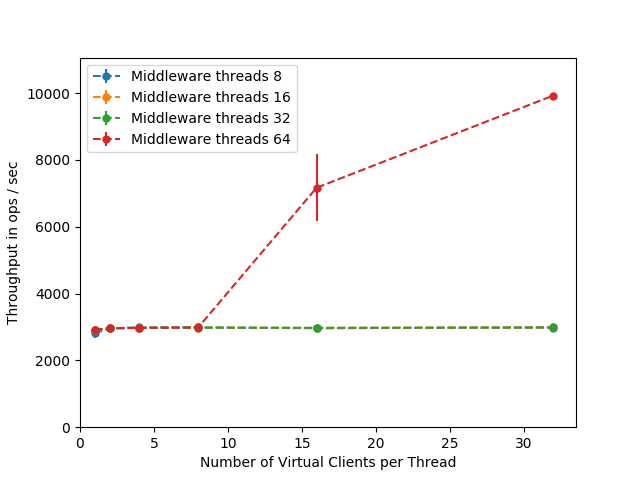
\includegraphics[width=\textwidth]{img/exp3_1/exp3_1__throughput_client_write_0.png}
    \caption{Throughput read only}
    \label{fig:mesh1}
\end{subfigure}
\caption{Exp3.1: Latency and throughputs as measures by the \textbf{clients}}
\label{fig:test}
\end{figure}

The client and middleware graphs deviate sligthly.
As one can see, the middleware graph seems more stable.
This is because the middleware graph only shows the performance \textbf{excluding} the warm-up and cool-down phase, whereas the client graphs do not exclude these measurements.

I now proceed with the same experiment but for write-only operations only.

\subsubsection{Write-only and Explanation}

\begin{figure}[H]
\centering
\begin{subfigure}{.5\textwidth}
    \centering
    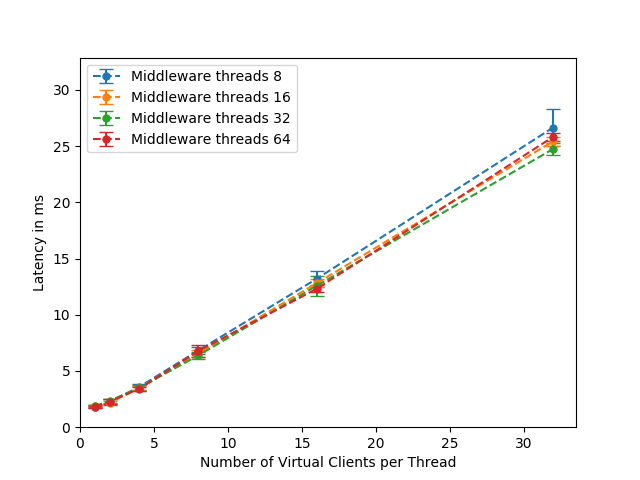
\includegraphics[width=\textwidth]{img/exp3_1/exp3_1__latency_client_write_1.png}
    \caption{Latency write only}
    \label{fig:mesh1}
\end{subfigure}%
\begin{subfigure}{.5\textwidth}
      \centering
    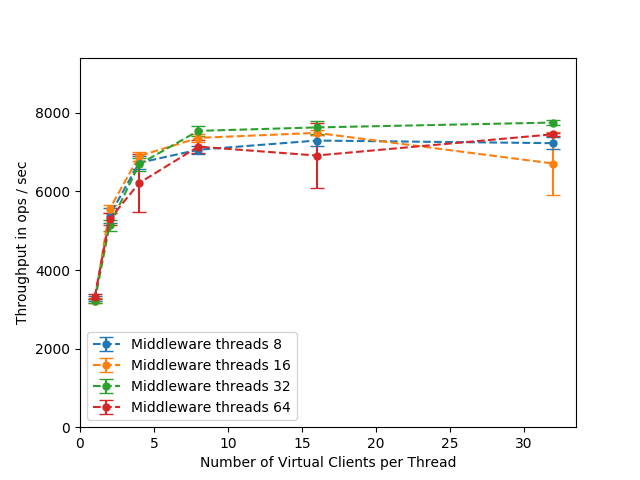
\includegraphics[width=\textwidth]{img/exp3_1/exp3_1__throughput_client_write_1.png}
    \caption{Throughput write only}
    \label{fig:mesh1}
\end{subfigure}
\caption{Exp3.1: Latency and throughputs as measures by the clients}
\label{fig:test}
\end{figure}


The single server is fast enough to respond to all individual client requests, as the server is only responding with the message "STORED" each time.
However, at some point, the number of requests is so high, that either the individual client output bandwidth, or storing the actual requests on the hard-ware side becomes the bottleneck.
This can be seen as the throughput grows square-root like, and then saturates.
The throughput graph, which means out with 16 virtual clients per thread, proves this point.
To decide whether the network is the bandwidth is the bottleneck, I repeat this experiment locally with virtual docker containers.
These plateau at a later stage, which proves that the maximum network bandwidth is reached with 16 virtual clients per thread.

%TODO :
Latency and throughput correlate in the following way: \textbf{???}

The following graphs are created using the logs of the client for the throughput and the latency, and underline that the values are sane.

As a sanity check, I present the throughput and latency plots from the client machines, which all conform to the throughputs and latencies as caluclated in the middleware.
Another sanity check is that the interactive law holds, which states that the response-time \textbf{per request}  is related inversely-linearly proportional to the throughput.


\begin{figure}[H]
\centering
\begin{subfigure}{.5\textwidth}
    \centering
    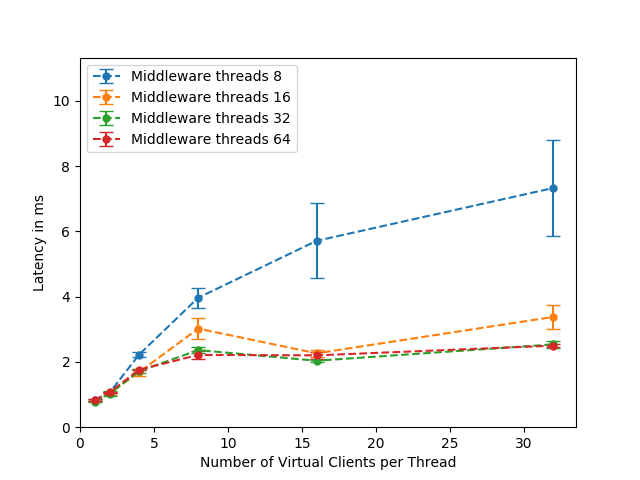
\includegraphics[width=\textwidth]{img/exp3_1/exp3_1__latency_middleware_write_1.png}
    \caption{Latency write only}
    \label{fig:mesh1}
\end{subfigure}%
\begin{subfigure}{.5\textwidth}
      \centering
    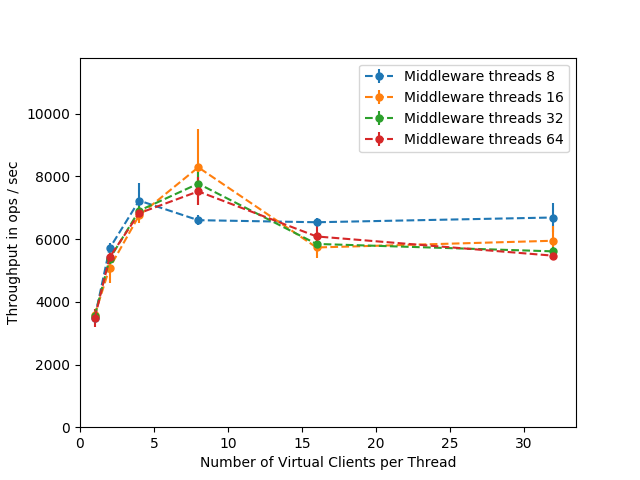
\includegraphics[width=\textwidth]{img/exp3_1/exp3_1__throughput_middleware_write_1.png}
    \caption{Throughput write only}
    \label{fig:mesh1}
\end{subfigure}
\caption{Exp3.1: Latency and throughputs as measures by the middlewares}
\label{fig:test}
\end{figure}

The client and middleware graphs deviate sligthly.
As one can see, the middleware graph seems more stable.
This is because the middleware graph only shows the performance \textbf{excluding} the warm-up and cool-down phase, whereas the client graphs do not exclude these measurements.

\subsubsection{Additional Explanation}

%TODO : compare read-only and write-only operations 

Provide a detailed analysis of the results (e.g., bottleneck analysis, component utilizations, average queue lengths, system saturation). Add any additional figures and experiments that help you illustrate your point and support your claims.

\subsection{Two Middlewares}

\begin{center}
	\scriptsize{
		\begin{tabular}{|l|c|}
			\hline Number of servers                & 1                        \\ 
			\hline Number of client machines        & 3                        \\ 
			\hline Instances of memtier per machine & 2                        \\ 
			\hline Threads per memtier instance     & 1                        \\
			\hline Virtual clients per thread       & [1..32]                  \\ 
			\hline Workload                         & Write-only and Read-only \\
			\hline Number of middlewares            & 2                        \\
			\hline Worker threads per middleware    & [8..64]                  \\
			\hline Repetitions                      & 3 or more (at least 1 minute each)                \\ 
			\hline 
		\end{tabular}
	} 
\end{center}

The setup is exactly the same as in experiment "Baseline without Middleware and 1 server", with the difference that we inject two middlewares between the clients, and the server.
Another difference is that we allow each individual client to run two memtier instances (each with one thread) to be able to connect to two instances each.
The throughput reached approximately almost $3000ops/s$, which conforms to the observation of the maximum throughput per server in section "Baseline without Middleware and 1 server". \\

In addition the measuring the throughput and response time for different values of number of virtual clients, we also allow to modify the number of middleware threads as another measureable variable.
This means that I test out the throughput and latency for any permutation of
virtualthreads=[1, 2, 4, 8, 16, 32] and threads in the middleware=[8, 16, 32, 64].
I repeat each experiment for 3 times and plot the standard deviation amongst those trials.
I also allow for a 15 second warm-up and 15 second cool-down time, and disregard these measurements when retrieving the logs about the request times from the middleware.\\

Connect three load generator machines (two instances of memtier with CT=1) to two middlewares and use 1 memcached server. Run a read-only and a write-only workload with increasing number of clients (between 2 and 64) and measure response time \emph{both at the client and at the middleware}, and plot the throughput and response time as measured in the middleware.

Repeat this experiment for different number of worker threads inside the middleware: 8, 16, 32, 64.

\begin{center}
	\scriptsize{
		\begin{tabular}{|l|c|}
			\hline Number of servers                & 1                        \\ 
			\hline Number of client machines        & 3                        \\ 
			\hline Instances of memtier per machine & 2                        \\ 
			\hline Threads per memtier instance     & 1                        \\
			\hline Virtual clients per thread       & [1..32]                  \\ 
			\hline Workload                         & Write-only and Read-only \\
			\hline Multi-Get behavior               & N/A                      \\
			\hline Multi-Get size                   & N/A                      \\
			\hline Number of middlewares            & 2                        \\
			\hline Worker threads per middleware    & [8..64]                  \\
			\hline Repetitions                      & 3 or more (at least 1 minute each)                \\ 
			\hline 
		\end{tabular}
	} 
\end{center}

\subsubsection{Read-only}

\begin{figure}[H]
\centering
\begin{subfigure}{.5\textwidth}
    \centering
    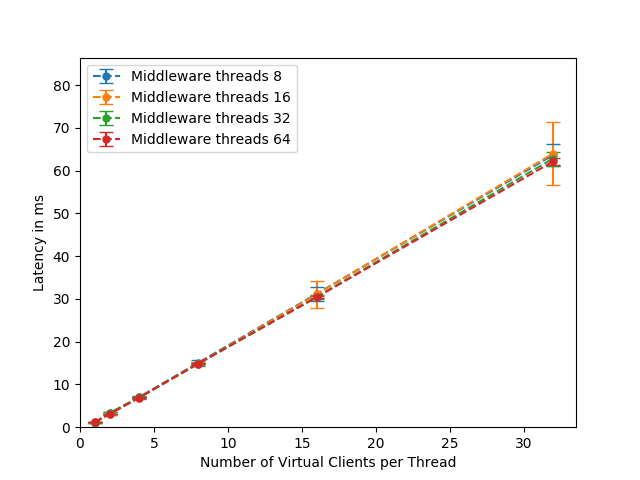
\includegraphics[width=\textwidth]{img/exp3_2/exp3_2__latency_middleware_write_0.png}
    \caption{Latency read only}
    \label{fig:mesh1}
\end{subfigure}%
\begin{subfigure}{.5\textwidth}
      \centering
    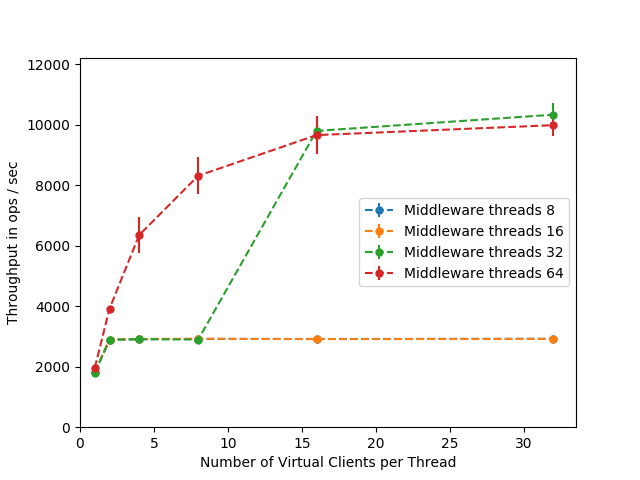
\includegraphics[width=\textwidth]{img/exp3_2/exp3_2__throughput_middleware_write_0.png}
    \caption{Throughput read only}
    \label{fig:mesh1}
\end{subfigure}
\caption{Exp3.2: Latency and throughputs as measures by the middlewares}
\label{fig:test}
\end{figure}

%TODO : explanation

\begin{figure}[H]
\centering
\begin{subfigure}{.5\textwidth}
    \centering
    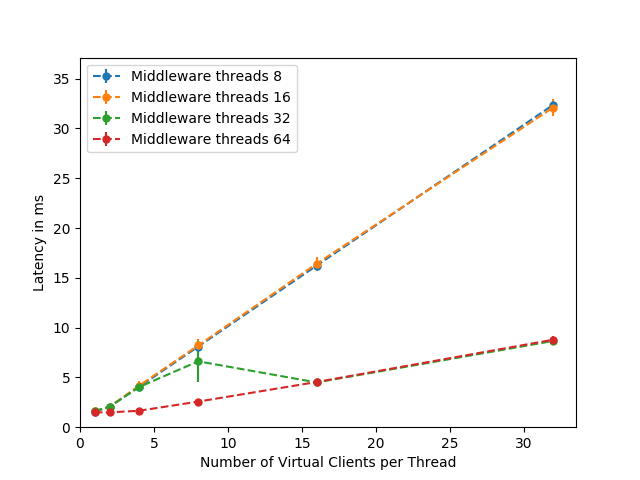
\includegraphics[width=\textwidth]{img/exp3_2/exp3_2__latency_client_write_0.png}
    \caption{Latency read only}
    \label{fig:mesh1}
\end{subfigure}%
\begin{subfigure}{.5\textwidth}
      \centering
    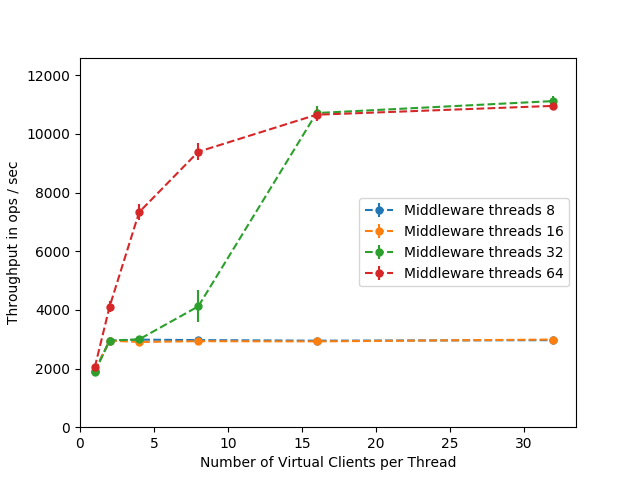
\includegraphics[width=\textwidth]{img/exp3_2/exp3_2__throughput_client_write_0.png}
    \caption{Throughput read only}
    \label{fig:mesh1}
\end{subfigure}
\caption{Exp3.2: Latency and throughputs as measures by the clients}
\label{fig:test}
\end{figure}

The client and middleware graphs deviate sligthly.
As one can see, the middleware graph seems more stable.
This is because the middleware graph only shows the performance \textbf{excluding} the warm-up and cool-down phase, whereas the client graphs do not exclude these measurements.


\subsubsection{Write-only}

\begin{figure}[H]
\centering
\begin{subfigure}{.5\textwidth}
    \centering
    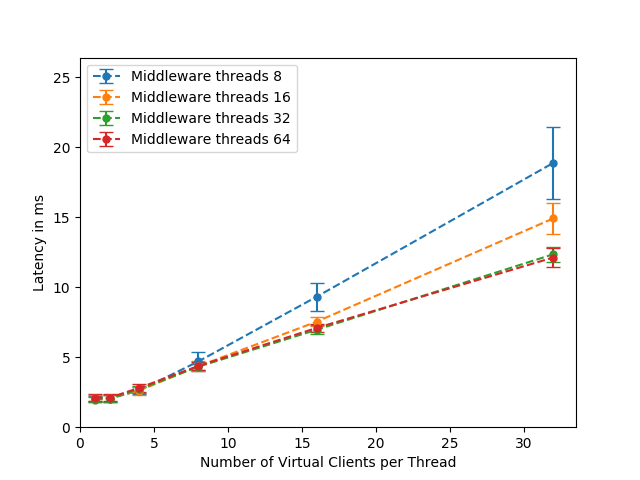
\includegraphics[width=\textwidth]{img/exp3_2/exp3_2__latency_client_write_1.png}
    \caption{Latency write only}
    \label{fig:mesh1}
\end{subfigure}%
\begin{subfigure}{.5\textwidth}
      \centering
    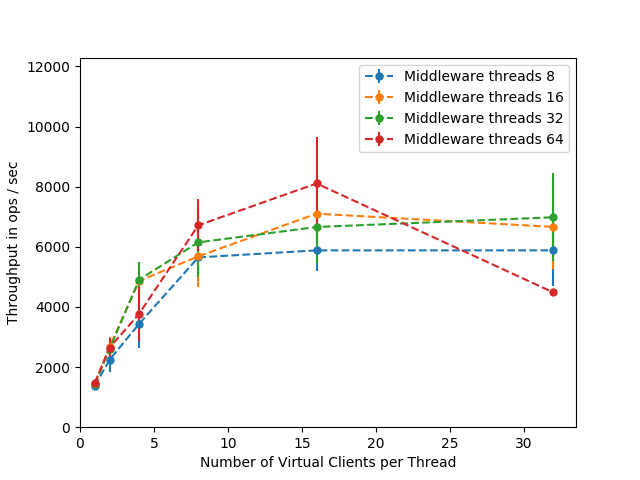
\includegraphics[width=\textwidth]{img/exp3_2/exp3_2__throughput_client_write_1.png}
    \caption{Throughput write only}
    \label{fig:mesh1}
\end{subfigure}
\caption{Exp3.2: Latency and throughputs as measures by the clients}
\label{fig:test}
\end{figure}

%TODO : explanation

\begin{figure}[H]
\centering
\begin{subfigure}{.5\textwidth}
    \centering
    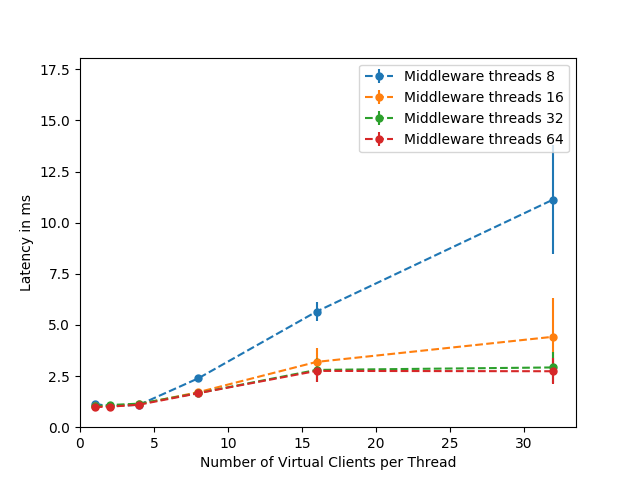
\includegraphics[width=\textwidth]{img/exp3_2/exp3_2__latency_middleware_write_1.png}
    \caption{Latency write only}
    \label{fig:mesh1}
\end{subfigure}%
\begin{subfigure}{.5\textwidth}
      \centering
    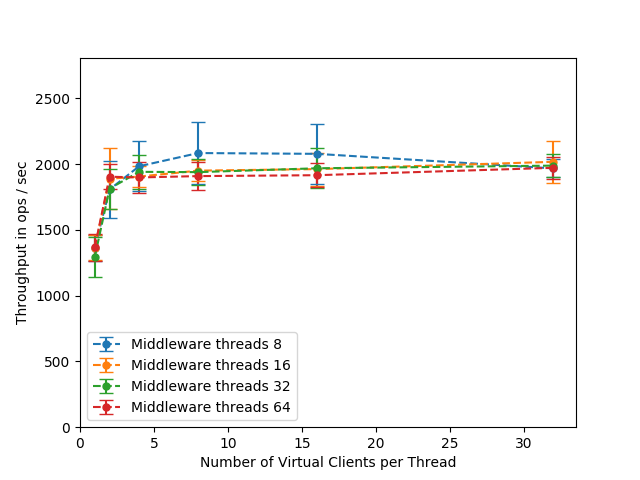
\includegraphics[width=\textwidth]{img/exp3_2/exp3_2__throughput_middleware_write_1.png}
    \caption{Throughput write only}
    \label{fig:mesh1}
\end{subfigure}
\caption{Exp3.2: Latency and throughputs as measures by the middlewares}
\label{fig:test}
\end{figure}

The client and middleware graphs deviate sligthly.
As one can see, the middleware graph seems more stable.
This is because the middleware graph only shows the performance \textbf{excluding} the warm-up and cool-down phase, whereas the client graphs do not exclude these measurements.

\subsubsection{Explanation}

Provide a detailed analysis of the results (e.g., bottleneck analysis, component utilizations, average queue lengths, system saturation). Add any additional figures and experiments that help you illustrate your point and support your claims.

\subsection{Summary}

Based on the experiments above, fill out the following table. For both of them use the numbers from a single experiment to fill out all lines. Miss rate represents the percentage of GET requests that return no data. Time in the queue refers to the time spent in the queue between the net-thread and the worker threads.


\begin{center}
	{Maximum throughput for one middleware.}
	\begin{tabular}{|l|p{2cm}|p{2cm}|p{2cm}|p{2cm}|}
		\hline                                & Throughput & Response time & Average time in queue & Miss rate \\ 
		\hline Reads: Measured on middleware  & 2933 & 64 &                       &           0 \\ 
		\hline Reads: Measured on clients     & 2987 & 64 & n/a                   &           0 \\ 
		\hline Writes: Measured on middleware & 8291 & 7 &                       & n/a       \\ 
		\hline Writes: Measured on clients    & 7423 & 34 & n/a                   & n/a       \\ 
		\hline 
	\end{tabular}
\end{center}

\begin{center}
	{Maximum throughput for two middlewares.}
	\begin{tabular}{|l|p{2cm}|p{2cm}|p{2cm}|p{2cm}|}
		\hline                                & Throughput & Response time & Average time in queue & Miss rate \\ 
		\hline Reads: Measured on middleware  & 10330 & 31.40 &                       &           0\\ 
		\hline Reads: Measured on clients     & 11116 &  32.37 & n/a                   &           0\\ 
		\hline Writes: Measured on middleware & 8131 & 11.13 &                       & n/a       \\ 
		\hline Writes: Measured on clients    & 8108 & 14.27 & n/a                   & n/a       \\ 
		\hline 
	\end{tabular}
\end{center}

Notice that the miss rate is always zero, because this is 1. a closed system, and all servers are pre-populated before any experiment starts.

Based on the data provided in these tables, write at least two paragraphs summarizing your findings about the performance of the middleware in the baseline experiments.

\section{Throughput for Writes (90 pts)}

\subsection{Full System}

Connect three load generating VMs to two middlewares and three memchached servers. Run a write-only experiment. 
You need to plot throughput and response time measured on the middleware as a function of number of clients. The measurements have to be performed for 8, 16, 32 and 64 worker threads inside each middleware.

This experiment only consists of write-only operations, so we don't subdivide this experiment into "write-only" and "read-only".

\begin{figure}[H]
\centering
\begin{subfigure}{.5\textwidth}
    \centering
    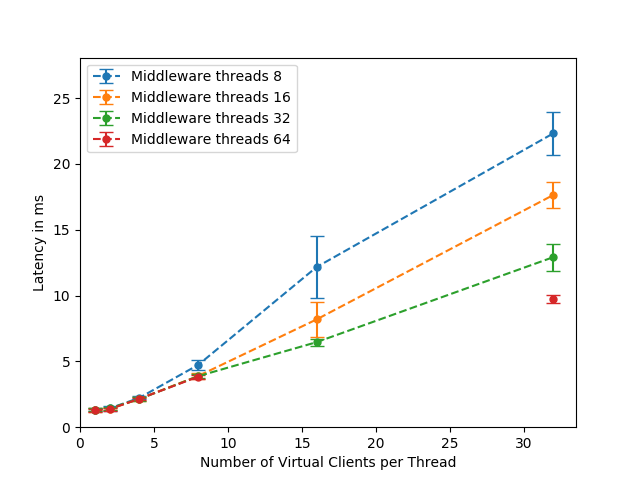
\includegraphics[width=\textwidth]{img/exp4_1/exp4_1__vc_64__latency_middleware_write_1.png}
    \caption{Latency write only}
    \label{fig:mesh1}
\end{subfigure}%
\begin{subfigure}{.5\textwidth}
      \centering
    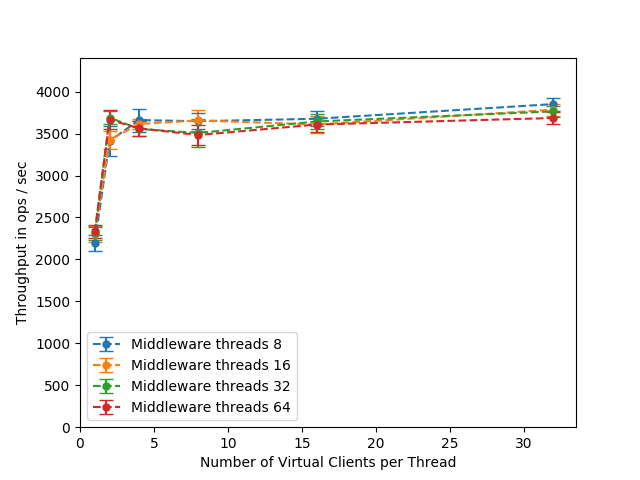
\includegraphics[width=\textwidth]{img/exp4_1/exp4_1__vc_64__throughput_middleware_write_1.png}
    \caption{Throughput write only}
    \label{fig:mesh1}
\end{subfigure}
\caption{Exp3.2: Latency and throughputs as measures by the middlewares}
\label{fig:test}
\end{figure}

\begin{figure}[H]
\centering
\begin{subfigure}{.5\textwidth}
    \centering
    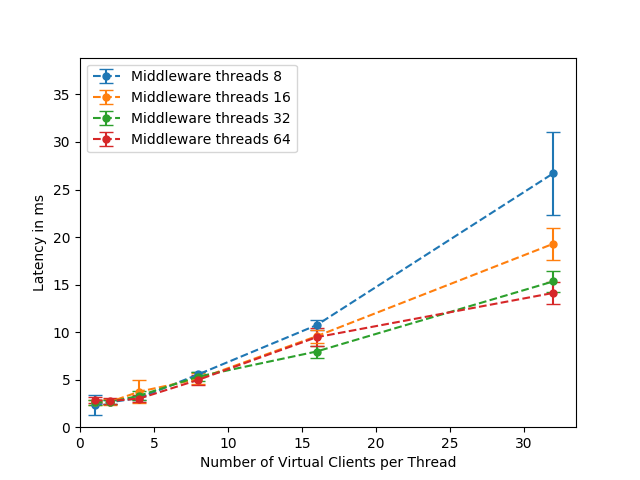
\includegraphics[width=\textwidth]{img/exp4_1/exp4_1__vc_64__latency_client_write_1.png}
    \caption{Latency write only}
    \label{fig:mesh1}
\end{subfigure}%
\begin{subfigure}{.5\textwidth}
      \centering
    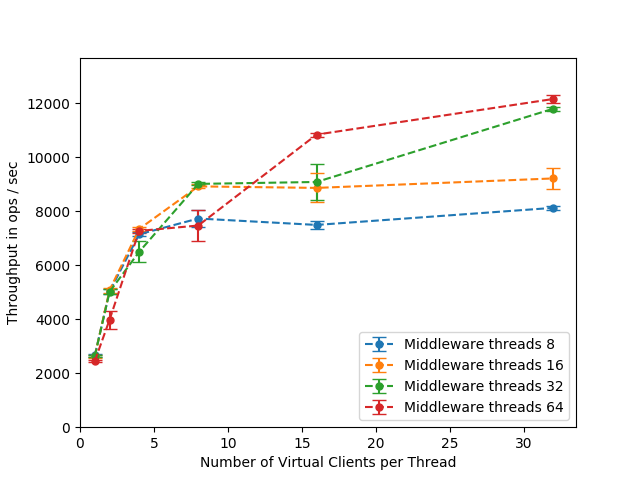
\includegraphics[width=\textwidth]{img/exp4_1/exp4_1__vc_64__throughput_client_write_1.png}
    \caption{Throughput write only}
    \label{fig:mesh1}
\end{subfigure}
\caption{Exp3.2: Latency and throughputs as measures by the clients}
\label{fig:test}
\end{figure}


\begin{center}
	\scriptsize{
		\begin{tabular}{|l|c|}
			\hline Number of servers                & 3          \\ 
			\hline Number of client machines        & 3          \\ 
			\hline Instances of memtier per machine & 2          \\ 
			\hline Threads per memtier instance     & 1          \\
			\hline Virtual clients per thread       & [1..32]    \\ 
			\hline Workload                         & Write-only \\
			\hline Multi-Get behavior               & N/A        \\
			\hline Multi-Get size                   & N/A        \\
			\hline Number of middlewares            & 2          \\
			\hline Worker threads per middleware    & [8..64]    \\
			\hline Repetitions                      & 3 or more (at least 1 minute each)  \\ 
			\hline 
		\end{tabular}
	} 
\end{center}

\subsubsection{Explanation}

Provide a detailed analysis of the results (e.g., bottleneck analysis, component utilizations, average queue lengths, system saturation). Add any additional figures and experiments that help you illustrate your point and support your claims.

\subsection{Summary}

Based on the experiments above, fill out the following table with the data corresponding to the maximum throughput point for all four worker-thread scenarios.

\begin{center}
	{Maximum throughput for the full system}
	\begin{tabular}{|l|p{1.5cm}|p{1.5cm}|p{1.5cm}|p{1.5cm}|}
		\hline                                            & WT=8 & WT=16 & WT=32 & WT=64 \\ 
		\hline Throughput (Middleware)                    & 14365 & 18338 & 18828 & 17984 \\ 
		\hline Throughput (Derived from MW response time) & 14632 & 18827 & 18504 & 17830  \\ 
		\hline Throughput (Client)                     &14858 & 17017 & 15703 & 17503 \\ 
		\hline Average time in queue                      &      &       &       &       \\ 
		\hline Average length of queue                    &      &       &       &       \\ 
		\hline Average time waiting for memcached         &      &       &       &       \\ 
		\hline 
	\end{tabular}
\end{center}

Based on the data provided in these tables, draw conclusions on the state of your system for a variable number of worker threads.

\section{Gets and Multi-gets (90 pts)}

For this set of experiments you will use three load generating machines, two middlewares and three memcached servers. Each memtier instance should have 2 virtual clients in total and the number of middleware worker threads is 64, or the one that provides the highest throughput in your system (whichever number of threads is smaller).

For multi-GET workloads, use the \texttt{--ratio} parameter to specify the exact ratio between SETs and GETs. You will have to measure response time on the client as a function of multi-get size, with and without sharding on the middlewares.

\subsection{Sharded Case}

Run multi-gets with 1, 3, 6 and 9 keys (memtier configuration) with sharding enabled (multi-gets are broken up into smaller multi-gets and spread across servers). Plot average response time as measured on the client, as well as the 25th, 50th, 75th, 90th and 99th percentiles.

\begin{center}
	\scriptsize{
		\begin{tabular}{|l|c|}
			\hline Number of servers                & 3                       \\ 
			\hline Number of client machines        & 3                       \\ 
			\hline Instances of memtier per machine & 2                       \\ 
			\hline Threads per memtier instance     & 1                       \\
			\hline Virtual clients per thread       & 2     		            \\ 
			\hline Workload                         & ratio=1:$<$Multi-Get size$>$             \\
			\hline Multi-Get behavior               & Sharded                 \\
			\hline Multi-Get size                   & [1..9]                  \\
			\hline Number of middlewares            & 2                       \\
			\hline Worker threads per middleware    & max. throughput config. \\
			\hline Repetitions                      & 3 or more (at least 1 minute each)               \\ 
			\hline 
		\end{tabular}
	} 
\end{center}

\begin{figure}[H]
\centering
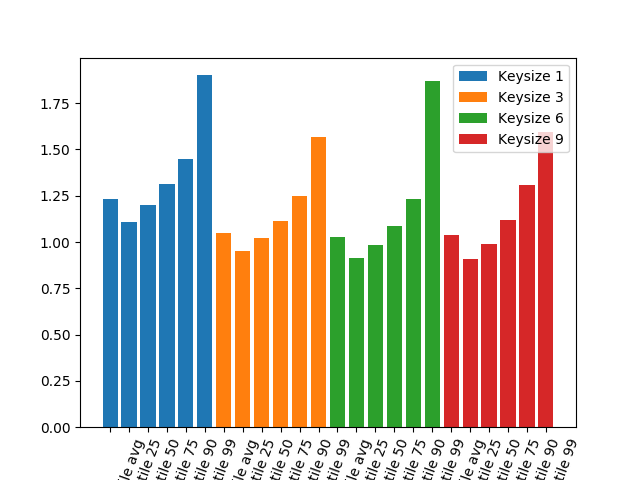
\includegraphics[width=\textwidth]{img/exp5_1/exp5_1_percentile_plots_sharded_True.png}
\caption{Exp3.2: Latency and throughputs as measures by the middlewares}
\label{fig:test}
\end{figure}

\begin{figure}[H]
\centering
\begin{subfigure}{.5\textwidth}
    \centering
    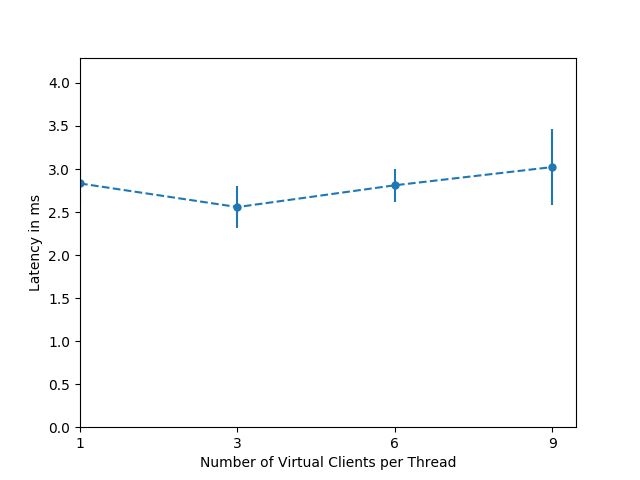
\includegraphics[width=\textwidth]{img/exp5_1/exp5_1__client_latency_sharding_True.png}
    \caption{Latency write only}
    \label{fig:mesh1}
\end{subfigure}%
\begin{subfigure}{.5\textwidth}
      \centering
    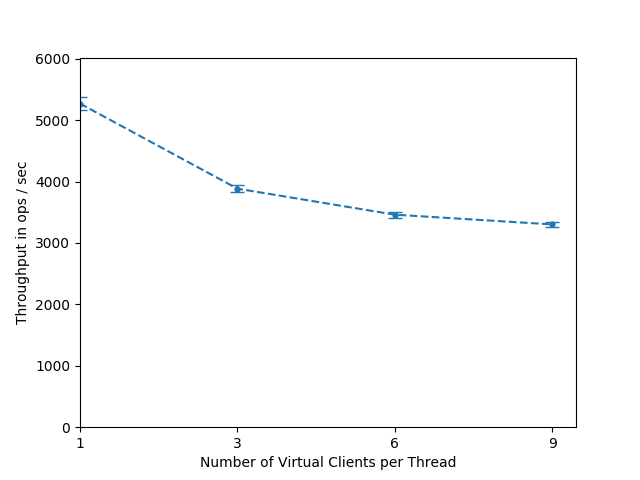
\includegraphics[width=\textwidth]{img/exp5_1/exp5_1__client_throughput_sharding_True.png}
    \caption{Throughput write only}
    \label{fig:mesh1}
\end{subfigure}
\caption{Exp3.2: Latency and throughputs as measures by the clients}
\label{fig:test}
\end{figure}

\begin{figure}[H]
\centering
\begin{subfigure}{.5\textwidth}
    \centering
    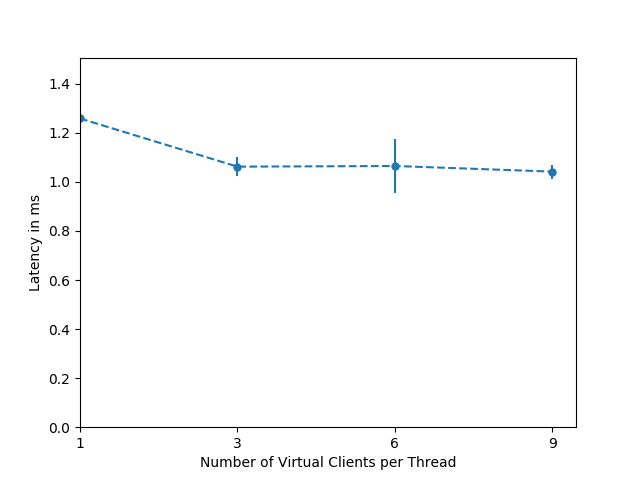
\includegraphics[width=\textwidth]{img/exp5_1/exp5_1__mw_latency_sharding_True.png}
    \caption{Latency write only}
    \label{fig:mesh1}
\end{subfigure}%
\begin{subfigure}{.5\textwidth}
      \centering
    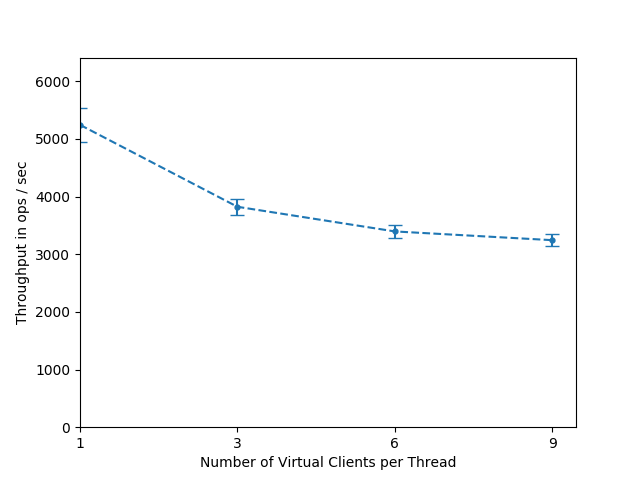
\includegraphics[width=\textwidth]{img/exp5_1/exp5_1__mw_throughput_sharding_True.png}
    \caption{Throughput write only}
    \label{fig:mesh1}
\end{subfigure}
\caption{Exp3.2: Latency and throughputs as measures by the middlewares}
\label{fig:test}
\end{figure}


\subsubsection{Explanation}

Provide a detailed analysis of the results (e.g., bottleneck analysis, component utilizations, average queue lengths, system saturation). Add any additional figures and experiments that help you illustrate your point and support your claims.

\subsection{Non-sharded Case}

Run multi-gets with 1, 3, 6 and 9 keys (memtier configuration) with sharding disabled. Plot average response time as measured on the client, as well as the 25th, 50th, 75th, 90th and 99th percentiles.

\begin{figure}[H]
\centering
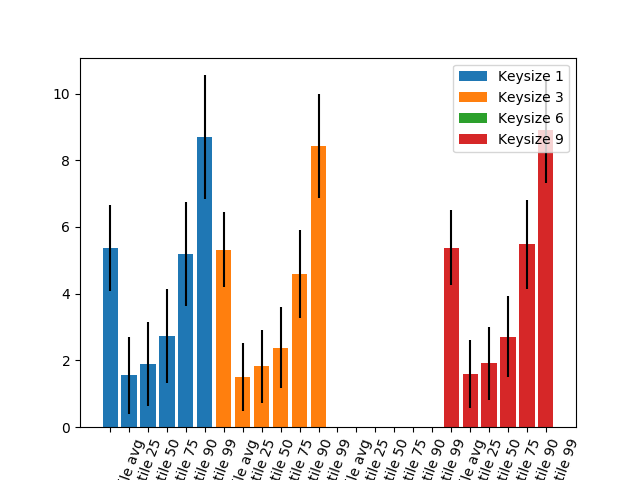
\includegraphics[width=\textwidth]{img/exp5_1/exp5_1_percentile_plots_sharded_False.png}
\caption{Exp3.2: Latency and throughputs as measures by the middlewares}
\label{fig:test}
\end{figure}

\begin{center}
	\scriptsize{
		\begin{tabular}{|l|c|}
			\hline Number of servers                & 3                       \\ 
			\hline Number of client machines        & 3                       \\ 
			\hline Instances of memtier per machine & 2                       \\ 
			\hline Threads per memtier instance     & 1                       \\
			\hline Virtual clients per thread       & 2                		 \\ 
			\hline Workload                         & ratio=1:$<$Multi-Get size$>$              \\
			\hline Multi-Get behavior               & Non-Sharded             \\
			\hline Multi-Get size                   & [1..9]                  \\
			\hline Number of middlewares            & 2                       \\
			\hline Worker threads per middleware    & max. throughput config. \\
			\hline Repetitions                      & 3 or more (at least 1 minute each)               \\ 
			\hline 
		\end{tabular}
	} 
\end{center}

\begin{figure}[H]
\centering
\begin{subfigure}{.5\textwidth}
    \centering
    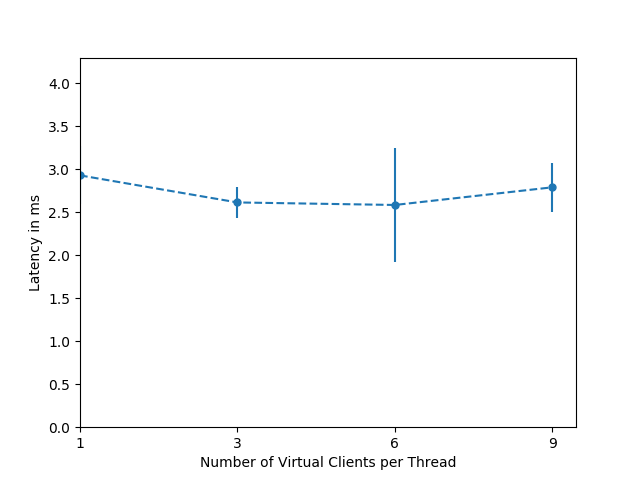
\includegraphics[width=\textwidth]{img/exp5_1/exp5_1__client_latency_sharding_False.png}
    \caption{Latency write only}
    \label{fig:mesh1}
\end{subfigure}%
\begin{subfigure}{.5\textwidth}
      \centering
    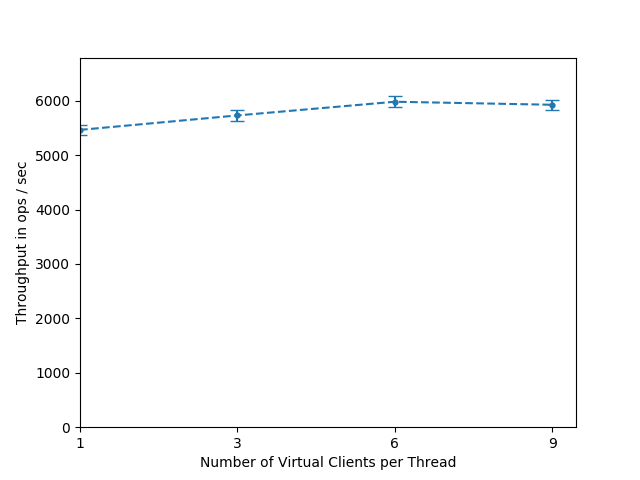
\includegraphics[width=\textwidth]{img/exp5_1/exp5_1__client_throughput_sharding_False.png}
    \caption{Throughput write only}
    \label{fig:mesh1}
\end{subfigure}
\caption{Exp3.2: Latency and throughputs as measures by the clients}
\label{fig:test}
\end{figure}

\begin{figure}[H]
\centering
\begin{subfigure}{.5\textwidth}
    \centering
    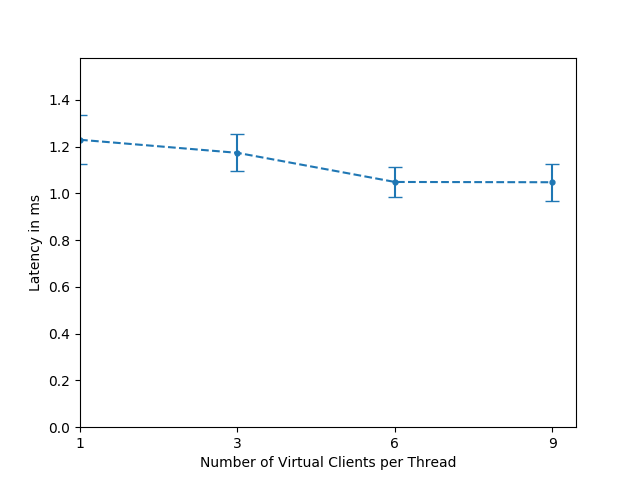
\includegraphics[width=\textwidth]{img/exp5_1/exp5_1__mw_latency_sharding_False.png}
    \caption{Latency write only}
    \label{fig:mesh1}
\end{subfigure}%
\begin{subfigure}{.5\textwidth}
      \centering
    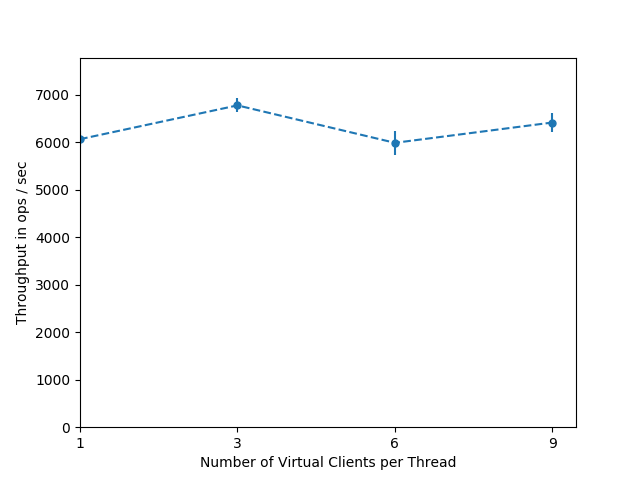
\includegraphics[width=\textwidth]{img/exp5_1/exp5_1__mw_throughput_sharding_False.png}
    \caption{Throughput write only}
    \label{fig:mesh1}
\end{subfigure}
\caption{Exp3.2: Latency and throughputs as measures by the middlewares}
\label{fig:test}
\end{figure}


\subsubsection{Explanation}

Provide a detailed analysis of the results (e.g., bottleneck analysis, component utilizations, average queue lengths, system saturation). Add any additional figures and experiments that help you illustrate your point and support your claims.

\subsection{Histogram}

For the case with 6 keys inside the multi-get, display four histograms representing the sharded and non-sharded response time distribution, both as measured on the client, and inside the middleware. Choose the bucket size in the same way for all four, and such that there are at least 10 buckets on each of the graphs.

\subsection{Summary}

Provide a detailed comparison of the sharded and non-shareded modes. For which multi-GET size is sharding the preferred option? Provide a detailed analysis of your system. Add any additional figures and experiments that help you illustrate your point and support your claims.

\section{2K Analysis (90 pts)}

This 2k analysis includes the analysis of any correlations between the following factors: 1. number of memcached servers, 2. the number of middleware vm's and finally 3. the number of worker threads per middleware.
The following table shows which possible values we cross-reference, such that we can later on analyse which factors have the most impact on throughput and response time.

\begin{itemize}
		
	\item Memcached servers: 1 and 3
	\item Middlewares: 1 and 2
	\item Worker threads per MW: 8 and 32
	      	      
\end{itemize}


Any configuration is run 3 times (3 repetitions) for 90 seconds, which implies a 15 second warm-up and a 15 second cool-down time.
The following table shows a detailed configuration of my setup.

\begin{center}
	\scriptsize{
		\begin{tabular}{|l|c|}
			\hline Number of servers                & 1 and 3                                     \\ 
			\hline Number of client machines        & 3                                           \\ 
			\hline Instances of memtier per machine & 1 (1 middleware) or 2 (2 middlewares) \\ 
			\hline Threads per memtier instance     & 2 (1 middleware) or 1 (2 middlewares)   \\
			\hline Virtual clients per thread       &  32                                     \\ 
			\hline Workload                         & Write-only and Read-only\\
			\hline Number of middlewares            & 1 and 2                                     \\
			\hline Worker threads per middleware    & 8 and 32                                    \\
			\hline Repetitions                      & 3 or more (at least 1 minute each)                                   \\ 
			\hline 
		\end{tabular}
	} 
\end{center}

I apply this analysis once for read-only workloads, and then separately for write-only workloads, as both procedures are fundamentally different.
I don't use any multi-get behavior (i.e. keysize is always 1 for read-only workloads). \\

For read-only and work-only workloads, I created tables which represent all possible configurations.
For both subsections, I will use the following abbreviations (and variable-names)

\begin{itemize}
\item NS: Number of Servers
\item NM: Number of Middlewares
\item WTMW: Worker threads per middleware
\end{itemize}

\subsubsection{Read-only}

% & Mean Latency 

\begin{center}
    \begin{tabular}{ | l | l | l | p{5cm} |}
    \hline
    NS (Servers) & NM (Middlewares) & WTMW (Workerthreads) & Mean Throughput \\ \hline
    1 & 1 & 8 & \\ \hline
    1& 1 & 32 & \\ \hline
    1 & 2 & 8 &  \\ \hline
   	1 & 2 & 32 & \\ \hline
    3 & 1 & 8 & \\ \hline
    3 & 1 & 32 &  \\ \hline
    3 & 2 & 8 &  \\ \hline
    3 & 2 & 32 &  \\
    \hline
    \end{tabular}
\end{center}

Repeat the experiment for (a)~a write-only and (b)~a read-only workload.
For each of the two workloads, what is the impact of these parameters on throughput, respectively response time?




\subsubsection{Write-only}



\section{Queuing Model (90 pts)}

In this section I model the workerqueue of the middleware (after the requests come in) using queueing theory to model how the system behaves with an asymptotically increasing number of threads.
In both subsection I will go use the different number of middleware (specifically, one of [8, 16, 32, 64]) threads to apply this analysis.

\subsection{M/M/1}
In this subsection I model the behavior of the middleware and it's workerqueue using a M/M/1 queueing model. \\

I choose the following input parameters to model the system:

First of all, I define the service rate to the model. 
For this, I look at the maximum throughput per number of middleware threads (amongst all given number of virtual clients). \\
From the file \textbf{create\_lineplot\_exp4\_1.py} I read out the respective maximum throughput values: \\

\begin{center}
	\scriptsize{
		\begin{tabular}{|l|c|}
			\hline Threads in the middleware & Maximum Throughput (ops/sec)                                     \\ 
			\hline 8 &   14365.88 \\ 
			\hline 16 &  18338.97 \\ 
			\hline 32 &  18828.88 \\
			\hline 64 &  17984.48 \\
			\hline
		\end{tabular}
	} 
\end{center}


your entire system. Motivate your choice of input parameters to the model. Explain for which experiments the predictions of the model match and for which they do not.

\subsection{M/M/m}

Build an M/M/m model based on Section 4, where each middleware worker thread is represented as one service.  Motivate your choice of input parameters to the model. Explain for which experiments the predictions of the model match and for which they do not.

\subsection{Network of Queues}

Based on Section 3, build a network of queues which simulates your system. Motivate the design of your network of queues and relate it wherever possible to a component of your system. Motivate your choice of input parameters for the different queues inside the network. Perform a detailed analysis of the utilization of each component and clearly state what the bottleneck of your system is. Explain for which experiments the predictions of the model match and for which they do not.

\end{document}